% Options for packages loaded elsewhere
\PassOptionsToPackage{unicode}{hyperref}
\PassOptionsToPackage{hyphens}{url}
\PassOptionsToPackage{dvipsnames,svgnames,x11names}{xcolor}
%
\documentclass[
  letterpaper,
  DIV=11,
  numbers=noendperiod]{scrreprt}

\usepackage{amsmath,amssymb}
\usepackage{iftex}
\ifPDFTeX
  \usepackage[T1]{fontenc}
  \usepackage[utf8]{inputenc}
  \usepackage{textcomp} % provide euro and other symbols
\else % if luatex or xetex
  \usepackage{unicode-math}
  \defaultfontfeatures{Scale=MatchLowercase}
  \defaultfontfeatures[\rmfamily]{Ligatures=TeX,Scale=1}
\fi
\usepackage{lmodern}
\ifPDFTeX\else  
    % xetex/luatex font selection
\fi
% Use upquote if available, for straight quotes in verbatim environments
\IfFileExists{upquote.sty}{\usepackage{upquote}}{}
\IfFileExists{microtype.sty}{% use microtype if available
  \usepackage[]{microtype}
  \UseMicrotypeSet[protrusion]{basicmath} % disable protrusion for tt fonts
}{}
\makeatletter
\@ifundefined{KOMAClassName}{% if non-KOMA class
  \IfFileExists{parskip.sty}{%
    \usepackage{parskip}
  }{% else
    \setlength{\parindent}{0pt}
    \setlength{\parskip}{6pt plus 2pt minus 1pt}}
}{% if KOMA class
  \KOMAoptions{parskip=half}}
\makeatother
\usepackage{xcolor}
\setlength{\emergencystretch}{3em} % prevent overfull lines
\setcounter{secnumdepth}{5}
% Make \paragraph and \subparagraph free-standing
\makeatletter
\ifx\paragraph\undefined\else
  \let\oldparagraph\paragraph
  \renewcommand{\paragraph}{
    \@ifstar
      \xxxParagraphStar
      \xxxParagraphNoStar
  }
  \newcommand{\xxxParagraphStar}[1]{\oldparagraph*{#1}\mbox{}}
  \newcommand{\xxxParagraphNoStar}[1]{\oldparagraph{#1}\mbox{}}
\fi
\ifx\subparagraph\undefined\else
  \let\oldsubparagraph\subparagraph
  \renewcommand{\subparagraph}{
    \@ifstar
      \xxxSubParagraphStar
      \xxxSubParagraphNoStar
  }
  \newcommand{\xxxSubParagraphStar}[1]{\oldsubparagraph*{#1}\mbox{}}
  \newcommand{\xxxSubParagraphNoStar}[1]{\oldsubparagraph{#1}\mbox{}}
\fi
\makeatother


\providecommand{\tightlist}{%
  \setlength{\itemsep}{0pt}\setlength{\parskip}{0pt}}\usepackage{longtable,booktabs,array}
\usepackage{calc} % for calculating minipage widths
% Correct order of tables after \paragraph or \subparagraph
\usepackage{etoolbox}
\makeatletter
\patchcmd\longtable{\par}{\if@noskipsec\mbox{}\fi\par}{}{}
\makeatother
% Allow footnotes in longtable head/foot
\IfFileExists{footnotehyper.sty}{\usepackage{footnotehyper}}{\usepackage{footnote}}
\makesavenoteenv{longtable}
\usepackage{graphicx}
\makeatletter
\newsavebox\pandoc@box
\newcommand*\pandocbounded[1]{% scales image to fit in text height/width
  \sbox\pandoc@box{#1}%
  \Gscale@div\@tempa{\textheight}{\dimexpr\ht\pandoc@box+\dp\pandoc@box\relax}%
  \Gscale@div\@tempb{\linewidth}{\wd\pandoc@box}%
  \ifdim\@tempb\p@<\@tempa\p@\let\@tempa\@tempb\fi% select the smaller of both
  \ifdim\@tempa\p@<\p@\scalebox{\@tempa}{\usebox\pandoc@box}%
  \else\usebox{\pandoc@box}%
  \fi%
}
% Set default figure placement to htbp
\def\fps@figure{htbp}
\makeatother
% definitions for citeproc citations
\NewDocumentCommand\citeproctext{}{}
\NewDocumentCommand\citeproc{mm}{%
  \begingroup\def\citeproctext{#2}\cite{#1}\endgroup}
\makeatletter
 % allow citations to break across lines
 \let\@cite@ofmt\@firstofone
 % avoid brackets around text for \cite:
 \def\@biblabel#1{}
 \def\@cite#1#2{{#1\if@tempswa , #2\fi}}
\makeatother
\newlength{\cslhangindent}
\setlength{\cslhangindent}{1.5em}
\newlength{\csllabelwidth}
\setlength{\csllabelwidth}{3em}
\newenvironment{CSLReferences}[2] % #1 hanging-indent, #2 entry-spacing
 {\begin{list}{}{%
  \setlength{\itemindent}{0pt}
  \setlength{\leftmargin}{0pt}
  \setlength{\parsep}{0pt}
  % turn on hanging indent if param 1 is 1
  \ifodd #1
   \setlength{\leftmargin}{\cslhangindent}
   \setlength{\itemindent}{-1\cslhangindent}
  \fi
  % set entry spacing
  \setlength{\itemsep}{#2\baselineskip}}}
 {\end{list}}
\usepackage{calc}
\newcommand{\CSLBlock}[1]{\hfill\break\parbox[t]{\linewidth}{\strut\ignorespaces#1\strut}}
\newcommand{\CSLLeftMargin}[1]{\parbox[t]{\csllabelwidth}{\strut#1\strut}}
\newcommand{\CSLRightInline}[1]{\parbox[t]{\linewidth - \csllabelwidth}{\strut#1\strut}}
\newcommand{\CSLIndent}[1]{\hspace{\cslhangindent}#1}

\KOMAoption{captions}{tableheading}
\makeatletter
\@ifpackageloaded{tcolorbox}{}{\usepackage[skins,breakable]{tcolorbox}}
\@ifpackageloaded{fontawesome5}{}{\usepackage{fontawesome5}}
\definecolor{quarto-callout-color}{HTML}{909090}
\definecolor{quarto-callout-note-color}{HTML}{0758E5}
\definecolor{quarto-callout-important-color}{HTML}{CC1914}
\definecolor{quarto-callout-warning-color}{HTML}{EB9113}
\definecolor{quarto-callout-tip-color}{HTML}{00A047}
\definecolor{quarto-callout-caution-color}{HTML}{FC5300}
\definecolor{quarto-callout-color-frame}{HTML}{acacac}
\definecolor{quarto-callout-note-color-frame}{HTML}{4582ec}
\definecolor{quarto-callout-important-color-frame}{HTML}{d9534f}
\definecolor{quarto-callout-warning-color-frame}{HTML}{f0ad4e}
\definecolor{quarto-callout-tip-color-frame}{HTML}{02b875}
\definecolor{quarto-callout-caution-color-frame}{HTML}{fd7e14}
\makeatother
\makeatletter
\@ifpackageloaded{bookmark}{}{\usepackage{bookmark}}
\makeatother
\makeatletter
\@ifpackageloaded{caption}{}{\usepackage{caption}}
\AtBeginDocument{%
\ifdefined\contentsname
  \renewcommand*\contentsname{Table of contents}
\else
  \newcommand\contentsname{Table of contents}
\fi
\ifdefined\listfigurename
  \renewcommand*\listfigurename{List of Figures}
\else
  \newcommand\listfigurename{List of Figures}
\fi
\ifdefined\listtablename
  \renewcommand*\listtablename{List of Tables}
\else
  \newcommand\listtablename{List of Tables}
\fi
\ifdefined\figurename
  \renewcommand*\figurename{Figure}
\else
  \newcommand\figurename{Figure}
\fi
\ifdefined\tablename
  \renewcommand*\tablename{Table}
\else
  \newcommand\tablename{Table}
\fi
}
\@ifpackageloaded{float}{}{\usepackage{float}}
\floatstyle{ruled}
\@ifundefined{c@chapter}{\newfloat{codelisting}{h}{lop}}{\newfloat{codelisting}{h}{lop}[chapter]}
\floatname{codelisting}{Listing}
\newcommand*\listoflistings{\listof{codelisting}{List of Listings}}
\makeatother
\makeatletter
\makeatother
\makeatletter
\@ifpackageloaded{caption}{}{\usepackage{caption}}
\@ifpackageloaded{subcaption}{}{\usepackage{subcaption}}
\makeatother

\usepackage{bookmark}

\IfFileExists{xurl.sty}{\usepackage{xurl}}{} % add URL line breaks if available
\urlstyle{same} % disable monospaced font for URLs
\hypersetup{
  pdftitle={Using Causal Questions for Theory Development},
  pdfauthor={D. Alex Hughes},
  colorlinks=true,
  linkcolor={blue},
  filecolor={Maroon},
  citecolor={Blue},
  urlcolor={Blue},
  pdfcreator={LaTeX via pandoc}}


\title{Using Causal Questions for Theory Development}
\author{D. Alex Hughes}
\date{2025-07-22}

\begin{document}
\maketitle

\renewcommand*\contentsname{Table of contents}
{
\hypersetup{linkcolor=}
\setcounter{tocdepth}{2}
\tableofcontents
}

\bookmarksetup{startatroot}

\chapter*{Learning Objectives}\label{learning-objectives}
\addcontentsline{toc}{chapter}{Learning Objectives}

\markboth{Learning Objectives}{Learning Objectives}

At the end of today's session, we should each be better able to:

\begin{enumerate}
\def\labelenumi{\arabic{enumi}.}
\tightlist
\item
  \textbf{Identify} the major theories in your discipline, and
  \textbf{apprecaite} the value in conversations informed by theory.
\item
  \textbf{Articulate} how your research question is informative of the
  major theories in your discipline.
\item
  \textbf{Recognize} that all theories have causal implications.
\item
  \textbf{Apply} the idea of the \emph{ideal experiment} as a dark
  mirror for theory understanding.
\end{enumerate}

\bookmarksetup{startatroot}

\chapter{Introductions}\label{introductions}

\section{Myself}\label{myself}

\section{Who 'Dis}\label{who-dis}

\begin{itemize}
\tightlist
\item
  Do you think of your professional work as belonging to:

  \begin{itemize}
  \tightlist
  \item
    A \emph{scientist}?
  \item
    A \emph{theorist}?
  \item
    An \emph{engineer}?
  \item
    Is there another descriptive label?
  \end{itemize}
\item
  What field are you writing in? Who would recognize your work?

  \begin{itemize}
  \tightlist
  \item
    One of the \emph{computer sciences}?
  \item
    One of the \emph{critical fields}?
  \item
    One of the \emph{social sciences}?
  \item
    One of the \emph{natural sciences}?
  \end{itemize}
\end{itemize}

\bookmarksetup{startatroot}

\chapter{Finding Theories}\label{finding-theories}

\begin{itemize}
\tightlist
\item
  The goal in this section is to move from the questions that we're
  researching to the theories that are running through our fields.
\item
  This is a strong claim, but no matter your field, whether it is a
  natural science, a social science, a journalistic field there are
  theories that are being looked at.
\end{itemize}

\section{Research Questions}\label{research-questions}

Many of us organize our research, and our talks which I saw early last
week, around research questions. They keep us from getting \emph{lost},
they keep our work \emph{organized,} the focus us on tasks that we can
actually complete.

But, you're doing the ✨\emph{fun ✨} work of your dissertation right
now! You're taking on three, or more, different tasks that are all
organized around a theme. That theme \emph{might as well be} a major
theory in your field!

This is how \textbf{books} come to be, and your dissertation is really a
first draft of your tenure book.

\section{Breakout One}\label{breakout-one}

\begin{tcolorbox}[enhanced jigsaw, titlerule=0mm, colback=white, toptitle=1mm, toprule=.15mm, bottomtitle=1mm, colframe=quarto-callout-note-color-frame, colbacktitle=quarto-callout-note-color!10!white, bottomrule=.15mm, leftrule=.75mm, opacityback=0, title=\textcolor{quarto-callout-note-color}{\faInfo}\hspace{0.5em}{Breakout 1}, opacitybacktitle=0.6, arc=.35mm, rightrule=.15mm, breakable, coltitle=black, left=2mm]

\begin{itemize}
\item
  Remind yourselves, what is the role of theory building in the
  cumulation of knowledge in the social sciences?
\item
  Is it important that what we know accumulates? If so, why? If not, why
  not?
\item
  What is your favorite social sciences textbook?
\end{itemize}

\end{tcolorbox}

\section{Can AI Accumulate
Knowledge?}\label{can-ai-accumulate-knowledge}

\begin{itemize}
\item
  Ralph, this morning, contended that it is, or might be possible, for
  AI to accumulate knowledge. That there is a way to systematize the
  process that we undertake as social scientists: to observe, abduct,
  place against known theory, and then produce hypotheses, and test
  those hypotheses?
\item
  Do you agree? Where are the points that you think an AI system is
  likely to be especially helpful in this process? Where are the points
  that you think an AI system is likely to be especially
  \emph{unhelpful} in the process?
\item
  If AI \emph{can} accumulate knowledge, and then produce new knowledge,
  should you be in this field --- academics --- right now? Should you be
  in this room right now?
\item
  I'm going to argue ``Yes'' even if AI can accumulate knowledge there's
  an important role for us --- what the machines have access to are
  probabilistic sets of words that belong together or in conversation;
  they can help us to understand what has been \emph{done} and what has
  been \emph{thought} --- but it does not have the capabilities (yet) to
  intervene and run trials or think counterfactually. \emph{At least for
  a little while, we're still ahead of the machines.}
\end{itemize}

\subsection{Discussion Questions}\label{discussion-questions}

\begin{tcolorbox}[enhanced jigsaw, titlerule=0mm, colback=white, toptitle=1mm, toprule=.15mm, bottomtitle=1mm, colframe=quarto-callout-note-color-frame, colbacktitle=quarto-callout-note-color!10!white, bottomrule=.15mm, leftrule=.75mm, opacityback=0, title=\textcolor{quarto-callout-note-color}{\faInfo}\hspace{0.5em}{1. Research Questions}, opacitybacktitle=0.6, arc=.35mm, rightrule=.15mm, breakable, coltitle=black, left=2mm]

Take a five minutes to write down for yourselves (it is OK for you to
use a LLM):

\begin{itemize}
\tightlist
\item
  What are the major \emph{questions} in your field?
\item
  This might require that you think back to your field exams! Try to
  think not about a specific study, but questions that many people who
  are working on.
\end{itemize}

\textbf{Examples:}

\begin{enumerate}
\def\labelenumi{\arabic{enumi}.}
\tightlist
\item
  Why does this apple fall from this tree, rather than floating away?
\item
  Why \emph{do}, and why \emph{don't}, citizens participate in electoral
  politics?
\item
  ``Misinformation''\ldots{} ?
\end{enumerate}

\end{tcolorbox}

What I think that we're going to see is that the major questions that
exist in the disparate fields are actually quite similar! Or, at least,
if you squint a little bit, the ways that we think of information access
among youth in Puerto Rico have to be related to the explanations news
production in Canada, and civic technology utilization in Georgia.

\bookmarksetup{startatroot}

\chapter{Answers to Research Questions are
Theories!}\label{answers-to-research-questions-are-theories}

As you're moving from questions being asked, toward some more general
explanation of phenomena, you're going to use our incredible, creative,
human ability to explain patterns with simpler stories. We do this
\emph{all. the. time.} Learning and abstraction, which I'm actively
seeing my child undertake on a daily basis, is one of the core human
super powers!

\begin{itemize}
\item
  We have burned ourselves on a fire ring at a campsight on the
  California coast. How quickly we're able to infer that a fire ring
  with an open flame in the Sierra Nevada mountains has the same
  properties, and will cause the same result, \emph{despite} being an
  entirely different location, context, elevation, and flame!
\item
  We have eaten cereal with cow's milk that has a certain off smell and
  feel ill afterwards. How quickly we are able to recognize that smell,
  and avoid products that have such a smell in the future. And! We're
  able to distinguish that smell of soured milk from the smells of
  cheeses, yogurts, and other similar cultured milk products.
\item
  We have grown up in the midwestern parts of the United States (or
  possibly other places, too) and know that when the weather changes
  rapidly from sunny to overcast, there is rain that is imminent.
\end{itemize}

\begin{tcolorbox}[enhanced jigsaw, titlerule=0mm, colback=white, toptitle=1mm, toprule=.15mm, bottomtitle=1mm, colframe=quarto-callout-note-color-frame, colbacktitle=quarto-callout-note-color!10!white, bottomrule=.15mm, leftrule=.75mm, opacityback=0, title=\textcolor{quarto-callout-note-color}{\faInfo}\hspace{0.5em}{Pattern Learning}, opacitybacktitle=0.6, arc=.35mm, rightrule=.15mm, breakable, coltitle=black, left=2mm]

\begin{itemize}
\item
  How can we learn patterns so quickly?
\item
  Are we ever wrong when we're learning these patterns? Are there times
  that the general rule that we see is incorrect? To broad? Too narrow?
\end{itemize}

\end{tcolorbox}

Are we generalizing knowledge --- called \emph{induction ---} or, are we
proposing what we believe to be the most likely explanation --- called
\emph{abduction}
(\href{https://plato.stanford.edu/entries/peirce/}{Charles Sanders
Pierce})?

\begin{tcolorbox}[enhanced jigsaw, titlerule=0mm, colback=white, toptitle=1mm, toprule=.15mm, bottomtitle=1mm, colframe=quarto-callout-note-color-frame, colbacktitle=quarto-callout-note-color!10!white, bottomrule=.15mm, leftrule=.75mm, opacityback=0, title=\textcolor{quarto-callout-note-color}{\faInfo}\hspace{0.5em}{2. Answers to Questions}, opacitybacktitle=0.6, arc=.35mm, rightrule=.15mm, breakable, coltitle=black, left=2mm]

Take five more minutes.

\begin{itemize}
\tightlist
\item
  What are the possible answers to these questions?
\item
  Which of these --- research questions, or theories --- are easier for
  you to find? Why?
\end{itemize}

\end{tcolorbox}

\begin{tcolorbox}[enhanced jigsaw, titlerule=0mm, colback=white, toptitle=1mm, toprule=.15mm, bottomtitle=1mm, colframe=quarto-callout-tip-color-frame, colbacktitle=quarto-callout-tip-color!10!white, bottomrule=.15mm, leftrule=.75mm, opacityback=0, title=\textcolor{quarto-callout-tip-color}{\faLightbulb}\hspace{0.5em}{Theoretical Answers}, opacitybacktitle=0.6, arc=.35mm, rightrule=.15mm, breakable, coltitle=black, left=2mm]

\begin{enumerate}
\def\labelenumi{\arabic{enumi}.}
\tightlist
\item
  Apples fall from trees with predictable paths and rates because apples
  are composed partially of earth and partially of water (rather than
  air or fire). Since things that are composed of either earth or water
  belong at the center of the universe, which is the center of the
  Earth, they fall toward where they rightfully belong (Aristotelian
  explanation.)
\item
  Citizens operate subject to resource and cognitive constraints and
  make trade offs between action and inaction that can be understood as
  noisy bets made by lazy thinkers.\\
\item
  \ldots?
\end{enumerate}

\end{tcolorbox}

\section{How do we notice these
patterns?}\label{how-do-we-notice-these-patterns}

\begin{tcolorbox}[enhanced jigsaw, titlerule=0mm, colback=white, toptitle=1mm, toprule=.15mm, bottomtitle=1mm, colframe=quarto-callout-note-color-frame, colbacktitle=quarto-callout-note-color!10!white, bottomrule=.15mm, leftrule=.75mm, opacityback=0, title=\textcolor{quarto-callout-note-color}{\faInfo}\hspace{0.5em}{Breakout: Noticing Questions and Answers}, opacitybacktitle=0.6, arc=.35mm, rightrule=.15mm, breakable, coltitle=black, left=2mm]

Take five minutes as a group to talk about: How, practically, do you go
about noticing the things that are interesting research questions; or,
the things that are likely explanations for answers to your research
questions?

Do you simply look around? Read widely in your field? Take baths and
ponder?

\end{tcolorbox}

\section{Theories are the proposed, sometimes incomplete, answers to
questions in your
field!}\label{theories-are-the-proposed-sometimes-incomplete-answers-to-questions-in-your-field}

A field of economics is concerned with the question, ``How do firms
work?'' which really means, ``How can a company get the most out of its
workers?''

Suppose that you are a plant manager in my home state of Michigan who
wants your plant to be as productive as possible.\footnote{Stretch your
  theory. Suppose that you're a lab manager who is managing post-docs
  and PhD students? Stretch further, you're an Associate Dean who wants
  to get the most out of your School/Department.}

You might think that people who aren't monitored will use the time that
they're not being watched to \emph{shirk}, which is to do work that is
of lower effort than you would like. (For a review of this question, see
\href{./field_experiments_with_firms.pdf}{Banidera, Barankay, Rasul
(2011).})

\textbf{How would reduce the amount of shirking?} (Tighter monitoring?
Monetary incentives for work completed? Social pressures from managers
who have monetary incentives? Social rewards for people who do
especially good work?)

An example of solution that cannot be experimented easily? Authority.

\section{Example: Perfect Pizza}\label{example-perfect-pizza}

This is going to age me, but there was a glorious moment, pre-pandemic,
where \emph{Bon Appetit} had won the internet.

Their YouTube had everything -- star power, shiny production, and a
connection to something that is important to everyone the world over --
\textbf{pizza!}

They conducted a series called ``Making Perfect.'' The goal was to make,
well, the \emph{Perfect Pizza} at home.

\url{https://www.youtube.com/watch?v=STpv0aTReIw}

\section{Perfect Pizza}\label{perfect-pizza}

What are the component of a perfect pizza?

Let's think through that exercise together. What would make the
\emph{perfect pizza?} How would you approach it? How would you describe
it?

\section{Finding Theories that
Matter}\label{finding-theories-that-matter}

Here's the hard part: When, or what, is the tradeoff between (a) working
within an existing theory and finding (another) ``novel'' test of that
theory that is going to contribute to the cumulation of knowledge (which
Ralph said rather woefully are written, but never cited); or, (b)
challenge a theory to produce a revision, change, adaptation, or
``notch'' in the evidence consistent with the theory that is meaningful?

\begin{tcolorbox}[enhanced jigsaw, titlerule=0mm, colback=white, toptitle=1mm, toprule=.15mm, bottomtitle=1mm, colframe=quarto-callout-note-color-frame, colbacktitle=quarto-callout-note-color!10!white, bottomrule=.15mm, leftrule=.75mm, opacityback=0, title=\textcolor{quarto-callout-note-color}{\faInfo}\hspace{0.5em}{Open Discussion}, opacitybacktitle=0.6, arc=.35mm, rightrule=.15mm, breakable, coltitle=black, left=2mm]

Should you try and \emph{time} your contribution so that you're working
on something that is hot when you're on the market? So you can be a
superstar on that junior search cycle?

Or, should you work on the theories that you think are interesting, no
matter if they're in a backwaters that are largely irrelevant to your
field?

What are the tradeoffs that you see as 4th year PhD?

\end{tcolorbox}

\bookmarksetup{startatroot}

\chapter{Theories to Questions}\label{theories-to-questions}

Ok, so we can move from questions to theories. How do we go the other
way around, and why is this important?

\bookmarksetup{startatroot}

\chapter{Theories to Questions}\label{theories-to-questions-1}

\section{Answers to Questions Separate
Theories}\label{answers-to-questions-separate-theories}

If you propose things \emph{work} differently than the field currently
believes, you're going to have to convince the field. And, it is
important to remember -- the field doesn't like to change its mind.
Researchers have reputations, and grants, that they intend to retain.
Even if your work is simply directed at the concepts, there will be
\emph{human-level} resistance to what you're proposing.

And so, if you've got this uphill battle to change the minds of your
discipline, how do you do it most effectively?

\begin{tcolorbox}[enhanced jigsaw, titlerule=0mm, colback=white, toptitle=1mm, toprule=.15mm, bottomtitle=1mm, colframe=quarto-callout-note-color-frame, colbacktitle=quarto-callout-note-color!10!white, bottomrule=.15mm, leftrule=.75mm, opacityback=0, title=\textcolor{quarto-callout-note-color}{\faInfo}\hspace{0.5em}{Changing Minds: Part 1}, opacitybacktitle=0.6, arc=.35mm, rightrule=.15mm, breakable, coltitle=black, left=2mm]

How do you best structure your argument/book to be most effective at
changing the minds of your field? How do you make it so they \emph{have}
\emph{to} engage with what you've written? What is the role of logical
deduction in this process?

\end{tcolorbox}

\section{\texorpdfstring{Theory \(\rightarrow\)
Hypotheses}{Theory \textbackslash rightarrow Hypotheses}}\label{theory-rightarrow-hypotheses}

\begin{quote}
\emph{``OK, I've got this theory. I think that \{these things\} \{do
this\} \{because of\} \{when that\}.''}
\end{quote}

\textbf{Now what?}

The process to go from your observations to the most likely set of
explanations --- the process of abduction --- is one of the steps that
produces the statement above 👆.

But, it cannot be the only step --- if that were the only step, we
wouldn't be social scientists; we'd be evangelists and zealots.

Because it is entirely within your own head it is fallible. Our minds'
ability to abstract events to patternss in amazing, but by its very
structure imprecise, and is it entirely possible that we might learn the
wrong generalization, or abduct what seems to be a reasonable
explanation but that is incorrect.

After all, when we're seeing some real-world event we're seeing it
within a limited context frame and that context shapes how or what might
occur. Although there are many, many explanations for why things occur,
there is almost certainly a boundless set of possible context frames
that we could have been within!

\section{Deductive Validity}\label{deductive-validity}

\textbf{Position}: Your goal, at some point in your dissertation, is to
produce a prediction that would be true \emph{if and only if} the theory
you believe to be the true explanation were in fact true.

Jeez. Let's unpack that.

First, recall that you're working within the \emph{enterprise} of
academic, and probably social scientific research. The people who are
working within the field carry forward the beliefs of their advisers
(and their advisers' advisers\ldots). And so, there are a lot of beliefs
out there --- a lot of explanations why things happened the way they
did.

In your dissertation work, and in the work that follows, you're taking a
position on how the world works. That's your job as a member of this
academy. But, your position is just one of many possible positions; and,
certainly, there will be other people who hold those other positions.
They're not straw-people positions, and there's little value in
positioning your work against such a staged argument.

\begin{tcolorbox}[enhanced jigsaw, titlerule=0mm, colback=white, toptitle=1mm, toprule=.15mm, bottomtitle=1mm, colframe=quarto-callout-note-color-frame, colbacktitle=quarto-callout-note-color!10!white, bottomrule=.15mm, leftrule=.75mm, opacityback=0, title=\textcolor{quarto-callout-note-color}{\faInfo}\hspace{0.5em}{Examples of Differing Positions}, opacitybacktitle=0.6, arc=.35mm, rightrule=.15mm, breakable, coltitle=black, left=2mm]

\begin{itemize}
\item
  Misinformation and disinformation are scourges that fundimentally
  threatens democratic accountability.
\item
  We've seen clear examples of the harms of misinformation and
  disinformation through the last several global election cycles. But,
  these are disequilibrium events and society will learn and develop
  ways to avoid such events in future states.
\end{itemize}

\end{tcolorbox}

Only one of those positions can be true --- either we're screwed, or
there are relatively minor fixes that we can enforce that will pull us
out of this morass. Which of these states of the world are we in, and
how would you know?

\textbf{Ask yourselves: ``Why?''} Why might we be fundamentally screwed?
What about humans' interactions with decentralized media create this
deep risk? \textbf{OR}, Why are there controls that we can actuate that
are likely to control the worst machinations of this political system?

\begin{tcolorbox}[enhanced jigsaw, titlerule=0mm, colback=white, toptitle=1mm, toprule=.15mm, bottomtitle=1mm, colframe=quarto-callout-note-color-frame, colbacktitle=quarto-callout-note-color!10!white, bottomrule=.15mm, leftrule=.75mm, opacityback=0, title=\textcolor{quarto-callout-note-color}{\faInfo}\hspace{0.5em}{Changing Minds: Part 2}, opacitybacktitle=0.6, arc=.35mm, rightrule=.15mm, breakable, coltitle=black, left=2mm]

How do you best structure your career to be most effective at changing
the minds of your field? How do you make it so they \emph{can} engage
with what you've written?

\end{tcolorbox}

\bookmarksetup{startatroot}

\chapter{Causal Implications}\label{causal-implications}

Here's a hot take for you:

🔥 Every (good) theory has a causal implication. 🔥

\section{What does it mean to cause?}\label{what-does-it-mean-to-cause}

There is a sub-field of language model training that is concerned with
teaching machines to learn what ``cause'' is. As it turns out\ldots{} it
continues to be a difficult task for machines to figure out.

As an example:

\begin{quote}
Lauren and Jane work for the same company. They each need to use a
computer for work sometimes. Unfortunately, the computer isn't very
powerful. If two people are logged on at the same time, it usually
crashes. So the company decided to institute an official policy. It
declared that Lauren would be the only one permitted to use the computer
in the mornings and that Jane would be the only one permitted to use the
computer in the afternoons. As expected, Lauren logged on the computer
the next day at 9:00 am. But Jane decided to disobey the official
policy. She also logged on at 9:00 am. The computer crashed immediately.
Did Jane cause the computer to crash?
\end{quote}

How do we think, as humans, think about this?

\section{Causal Thinking}\label{causal-thinking}

\begin{tcolorbox}[enhanced jigsaw, titlerule=0mm, colback=white, toptitle=1mm, toprule=.15mm, bottomtitle=1mm, colframe=quarto-callout-note-color-frame, colbacktitle=quarto-callout-note-color!10!white, bottomrule=.15mm, leftrule=.75mm, opacityback=0, title=\textcolor{quarto-callout-note-color}{\faInfo}\hspace{0.5em}{What does it mean for an action to \emph{cause} an outcome?}, opacitybacktitle=0.6, arc=.35mm, rightrule=.15mm, breakable, coltitle=black, left=2mm]

Literally, that's the prompt. What does it mean to cause?

Take five minutes to discuss that, and we'll come back.

\end{tcolorbox}

\subsection{Judea Pearl and DAGs}\label{judea-pearl-and-dags}

One of the systems, which Ralph has talked about this morning, is DAG
thinking --- derived from Judea Pearl's \emph{Causality (2000)?} In this
line of thinking, you write down all the concepts in the world, and you
draw the ``geometry'' of what you understand to cause what. Once you
write those down, you can reason about what you need to measure,
and\ldots{} \emph{Bob's Your Uncle.}

\begin{itemize}
\tightlist
\item
  What are the limitations of this approach?
\end{itemize}

\subsection{\texorpdfstring{Counterfactual Reasoning
(\href{https://www.jstor.org/stable/2245382?seq=1}{Neyman (1923)},
\href{https://web.archive.org/web/20170809031235id_/http://andrewmbailey.com/dkl/Counterfactuals_Comparative.pdf}{Lewis
(1973)}, \href{https://www.jstor.org/stable/pdf/2958688}{Rubin
(1978)})}{Counterfactual Reasoning (Neyman (1923), Lewis (1973), Rubin (1978))}}\label{counterfactual-reasoning-neyman-1923-lewis-1973-rubin-1978}

We employ counterfactual reasoning. This means that we think about one
circumstance where action would be taken, and we think about the
\emph{very same} outcome when the action would not be taken. In this
sense, there are two states of the world that are exactly the same but
with only a single difference.

If outcomes are different between these two states of the world, then we
say that the action causes the outcome.

\begin{tcolorbox}[enhanced jigsaw, titlerule=0mm, colback=white, toptitle=1mm, toprule=.15mm, bottomtitle=1mm, colframe=quarto-callout-note-color-frame, colbacktitle=quarto-callout-note-color!10!white, bottomrule=.15mm, leftrule=.75mm, opacityback=0, title=\textcolor{quarto-callout-note-color}{\faInfo}\hspace{0.5em}{What is the problem with this line of reasoning?}, opacitybacktitle=0.6, arc=.35mm, rightrule=.15mm, breakable, coltitle=black, left=2mm]

\begin{itemize}
\item
  Do you have a problem with this way of thinking?
\item
  Do you have a problem with using this as a way of producing evidence
  that is consistent with one theory and inconsistent with another
  theory?
\item
  How is what we have identified as a problem, actually an opportunity
  for us as academics to produce knowledge?
\end{itemize}

\end{tcolorbox}

\section{Finding Causes}\label{finding-causes}

How do we go about finding the antecedents (causes) and their
consequences (effects)?

These are the if-then squiggly lines that Ralph alluded to. The sets of
connections that undergird the realty that we exist within.

\begin{figure}[H]

{\centering \pandocbounded{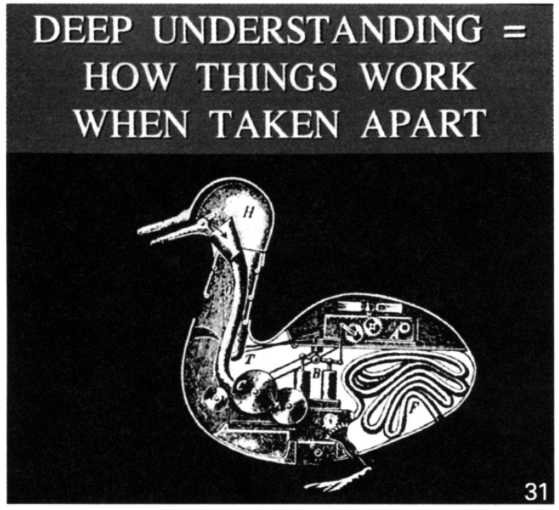
\includegraphics[keepaspectratio]{duck.png}}

}

\caption{What happens when we take things apart?}

\end{figure}%

\section{Theories that Don't Have Causal
Implications}\label{theories-that-dont-have-causal-implications}

\begin{itemize}
\tightlist
\item
  \textbf{Public Health?} Think about
  \href{https://en.wikipedia.org/wiki/Ronald_Fisher\#Contentious_views_on_smoking}{Ronald
  Fisher} --- would you die for your theory? He did! Public Health (not
  a social science, but instead a medical field that represents the
  worst of the social sciences\ldots) talks in terms of correlates of;
  determinants of; associates with.
\end{itemize}

\begin{figure}[H]

{\centering \pandocbounded{\includegraphics[keepaspectratio]{snow_map.jpeg}}

}

\caption{John Snow's Map of London, Showing Outbreaks of Choleara}

\end{figure}%

\begin{tcolorbox}[enhanced jigsaw, titlerule=0mm, colback=white, toptitle=1mm, toprule=.15mm, bottomtitle=1mm, colframe=quarto-callout-note-color-frame, colbacktitle=quarto-callout-note-color!10!white, bottomrule=.15mm, leftrule=.75mm, opacityback=0, title=\textcolor{quarto-callout-note-color}{\faInfo}\hspace{0.5em}{Discussion Question}, opacitybacktitle=0.6, arc=.35mm, rightrule=.15mm, breakable, coltitle=black, left=2mm]

Look back to the theories that you wrote down earlier --- are there any
of these, for which, you cannot imagine a causal implication?

\end{tcolorbox}

\bookmarksetup{startatroot}

\chapter{Ideal Experiments}\label{ideal-experiments}

Here's the thing --- you're probably a 4th year PhD student. Which
means\ldots{} 💸 👻 🏦

\ldots{} and running field experiments in the real world is
\emph{mind-bendingly expensive}. For example, experiments that Alex has
run in Guatemala (\$25M total program; \$1M experiment) and Pennsylvania
(\$2M total cost)

What's more --- you've probably already proposed your work to your
advisers and the worst outcome that could happen from this Summer
Doctoral Program is that you return to your institution, throw out your
work, and blame Eric, Ralph, David and Kimmy.

\textbf{But.} Can you imagine the ✨\textbf{ideal experiments ✨} that
you could conduct that would be consistent with your theory and
inconsistent with other theories?

\section{Ideal Experiment}\label{ideal-experiment}

The
\href{https://media4.giphy.com/media/v1.Y2lkPTc5MGI3NjExOGxha21yNXV4djg5NXh5bG9uMHpnNmhoOGV1MWt3aXhnM2h3Y3BwMyZlcD12MV9pbnRlcm5hbF9naWZfYnlfaWQmY3Q9dg/RtFGrL8Fn2xutS0qmN/giphy.gif}{\textbf{ideal
experiment}} is the experiment that you would conduct with:

\begin{itemize}
\item
  Unlimited Time
\item
  Perfect Measurement
\item
  Infinite Budget
\end{itemize}

There's a part of me that says, ``Well, that's easy if you've got
unlimited resources and perfect measurement.'' But, trust me, \emph{it
isn't.}..

The ideal experiment has to produce evidence that is consistent with one
theory but not consistent with any other theory; and it has to do so
\emph{cleanly}, that is, without complex causes (where more than one
feature moves at at time).

🙅The ideal experiment is \emph{not} concerned with: 🙅

\begin{itemize}
\item
  \textbf{Practical considerations}: it would be hard to\ldots{}
\item
  \textbf{Normative considerations}: it would create compensatory harm
  if one unit got \{this\} while the other unit got \{that\}
\item
  \textbf{Statistical considerations}: your focus is on the design and
  the relationship between the outcomes, intervention, and
  theory\ldots{} not on getting the model right. Hand-wave that model
  right out the door.
\end{itemize}

\section{Failure Points in Ideal
Experiments}\label{failure-points-in-ideal-experiments}

\begin{itemize}
\item
  \textbf{Your theory isn't precise enough.} While you've been building
  your explanation for ``why'' the world works, you've elided parts of
  the thinking that are necessary to produce a whole story. Imprecise
  theory produces bulky tests that don't actually have crisp
  predictions.
\item
  \textbf{Your theory overlaps too much with existing theories.} If you
  cannot produce a prediction that would be true \emph{if and only if}
  your theory were correct, you haven't made a contribution to the
  field!
\item
  \textbf{The other theories aren't precise enough\emph{.}} It isn't a
  problem of your creation, but it \emph{is} a problem that you've got
  to address. If the existing theory (``Prospect Theory'' anyone?) isn't
  sufficiently well developed, then it will overlap with your work.
\item
  \textbf{You don't know all the theories out there}. This is hard,
  you're a burgeoning professional, but you don't know everything!
  (Neither do I; Ralph and Eric may).
\end{itemize}

\bookmarksetup{startatroot}

\chapter*{References}\label{references}
\addcontentsline{toc}{chapter}{References}

\markboth{References}{References}

\phantomsection\label{refs}
\begin{CSLReferences}{0}{1}
\end{CSLReferences}




\end{document}
